	\documentclass[12pt,a4paper,headings=optiontohead]{article}
	\usepackage[utf8]{inputenc}
	\usepackage[italian]{babel}
	\usepackage[margin=1.8cm,bottom=7em]{geometry}
	\usepackage[subpreambles=false]{standalone}
	\usepackage{amsmath}
	\usepackage{amssymb}
	\usepackage{amsthm} 
	\usepackage{cancel}
	\usepackage{graphicx}
	\usepackage{mathtools}
	\usepackage{float}
	\usepackage{enumitem}
	\usepackage{algorithm}
	\usepackage{algorithmic}
	
	
	\usepackage[normalem]{ulem}
	
	\usepackage{blkarray}% http://ctan.org/pkg/blkarray
	
	\newcommand{\matindex}[1]{\mbox{\scriptsize#1}}% Matrix index
	
	\renewcommand{\qedsymbol}{\rule{0.7em}{0.7em}}
	\DeclarePairedDelimiter{\abs}{\lvert}{\rvert}
	\newcommand{\inter}{\begin{matrix}\prod\end{matrix}}
	\newcommand{\verteq}{\rotatebox{90}{$\,=$}}
	\newcommand{\equalto}[2]{\underset{\scriptstyle\overset{\mkern4mu\verteq}{#2}}{#1}}
	\DeclarePairedDelimiter{\norma}{\lVert}{\rVert}
	\newtheorem*{esempio}{Esempio}
	
	\usepackage{import}
	\usepackage{hyperref}
	\begin{document}
	
	%------------------------------------------------------------------------------------------------------
	%------------------------------------------------------------------------------------------------------
	%-----------------------------------------------INTESTAZIONE-------------------------------------------
	%------------------------------------------------------------------------------------------------------
	%------------------------------------------------------------------------------------------------------
	
	\begin{titlepage}
	
	\newcommand{\HRule}{\rule{\linewidth}{0.5mm}} % Defines a new command for the horizontal lines, change thickness here
	
	\center% Center everything on the page
	 
	%----------------------------------------------------------------------------------------
	%	HEADING SECTIONS
	%----------------------------------------------------------------------------------------
	
	
	
	
	
\includegraphics[height=4cm]{../img/btllogo.png}\\[0.3cm]
	%----------------------------------------------------------------------------------------
	%	TITLE SECTION
	%----------------------------------------------------------------------------------------
	
	\HRule \\[0.4cm]
	{ \huge \bfseries Relazione del progetto di}\\
	{ \huge \bfseries Tecnologie Web\\[0.15 cm]} % Title of your document
	\HRule \\[1.5cm]
	 
	%----------------------------------------------------------------------------------------
	%	AUTHOR SECTION
	%----------------------------------------------------------------------------------------
	\emph{\Large{Autori:}}\\
	\renewcommand{\arraystretch}{1.4}
	 \begin{center}
	 \begin{tabular}{r|l}	
		\textbf{Nominativo} & \textbf{Matricola}\\ \hline
	Antonio \textsc{Badan} & 1201209\\
	Simone \textsc{De Renzis} & 1187510\\
	Francesco \textsc{Trolese} & 1187224\\
	Luca \textsc{Veronese} & 1187571\\
	 \end{tabular}
	 \end{center}
	
	%----------------------------------------------------------------------------------------
	%	DATE SECTION
	% %----------------------------------------------------------------------------------------
	\vspace{1.5cm}
	{\LARGE Università degli Studi di Padova}\\[0.4cm] % Name of your university/college
	\textsc{\large{Dipartimento di Matematica}}\\[0.05cm]
	\textsc{\large{Corso di Laurea in Informatica}}\\[0.5cm]% Include a department/university logo - this will require the graphicx package
	{\Large Anno accademico 2020 - 2021}\\ % Date, change the \today to a set date if you want to be precise
	
	\vfill % Fill the rest of the page with whitespace
	
	
	
	\emph{\Large{Utenti preregistrati:}}\\
	
	\renewcommand{\arraystretch}{1.4}
	 \begin{center}
	 \begin{tabular}{|r|l|l|l|}
	 \hline
	\textbf{Utente} & \textbf{mail} & \textbf{Password} & \textbf{Categoria}  \\ \hline \hline
	 &  &  & \\ \hline
	
	 \end{tabular}
	 \end{center}
	
	\end{titlepage}
	
	
	\begin{center}
	\pagebreak
	
	\section*{Abstract}
	\begin{minipage}{0.9\textwidth} 
	\large{\textit{Between the Lines} è un sito di recensioni di libri che si pone l'obiettivo di raccogliere appassionati che condividono opinioni sulle loro letture.}
	\end{minipage}
	\end{center}
	\pagebreak
	
	\tableofcontents
	
	% ############ CAPITOLO 1 ##################
	\section{Analisi dei requisiti}
	
	Il sito Between The Lines vuol essere una piattaforma di incontro e condivisione di idee fra appassionati di libri e non. I lettori più accaniti possono esporre pensieri e valutazioni sui libri letti, indirizzando l'utente in cerca della prossima lettura verso un libro di proprio gradimento.
	
	
	\subsection{Attori}
	
	Le tipologie di utenti che interagiscono con il sito sono:
	\begin{itemize}
		\item \textbf{Utente generico}: non è registrato nel sito;
		\item \textbf{Utente registrato}: è registrato nel sito e vi accede con le proprie credenziali;
		\item \textbf{Utente Amministratore}: utente registrato con privilegi di amministrazione sul sito. \'E unico e non sono creabili nuovi account Amministratore. 
	\end{itemize} 
	
	
	\subsection{Funzionalità}
	
	\subsubsection{Tutti}
	Tutte le tipologie di utenti possono accedere al sito e usufruire delle funzionalità base di:
	\begin{itemize}
		\item \textbf{Ricerca}: una barra di ricerca permette di individuare il libro di proprio interesse tra i libri presenti nel catalogo. \'E possibile applicare dei filtri per discriminare se la ricerca avviene per Titolo o per Autore. \'E possibile ma non obbligatorio specificare un Genere. Questi accorgimenti danno la possibilità anche agli utenti che hanno un'idea meno chiara sulla lettura di individuare di esplorare le possibilità che offre il catalogo del sito;
		\item \textbf{Classifiche}: la pagina iniziale offre due sezioni che individuano i 3 libri più recensiti del catalogo, e le ultime 3 recensioni inserite. L'utente può immediatamente visualizzare quali siano i libri più popolari nella comunità di Between The Lines e orientare la propria scelta;
		\item \textbf{Dettagli del libro}: dopo una ricerca o tramite le classifiche, l'utente è indirizzato alla pagina di visualizzazione dei dettagli del libro: questa mostra in grande l'immagine di copertina del libro, i dettagli sull'autore e sul genere, e un breve riassunto della trama;
		\item \textbf{Visualizzare recensioni}: in fondo alla pagina sui dettagli del libro, sono presenti le recensioni degli utenti, ordinate in base alla data e ora di inserimento.
		\item \textbf{Contattare i creatori del sito}: la pagina Contatti presenta un form che permette di contattare i creatori del sito (visualizzabili nella pagina Chi siamo);
	\end{itemize}

	\subsubsection{Utente generico}

	L'utente generico può inoltre:
	\begin{itemize}
		\item \textbf{Registrarsi}: l'utente generico può entrare a far parte della comunità di Between the Lines.
	\end{itemize}
	
	\subsubsection{Utente registrato}
	
	L'utente registrato può:
	\begin{itemize}
		\item \textbf{Effettuare il login};
		\item \textbf{Inserire una recensione}: tramite apposito form a cui viene indirizzato dalla pagina dei dettagli del libro di cui vuole esprimere la propria opinione. La recensione si compone di una valutazione numerica sul gradimento del libro, e da un contenuto testuale. Ogni utente può inserire più di una recensione per ogni libro;
		\item \textbf{Eliminare una propria recensione}: tramite pulsante posto a fianco alla propria recensione;
		\item \textbf{Modificare i propri dati}: se loggato, l'utente può modificare i propri dati di registrazione al sito;
		\item \textbf{Effettuare il logout};
	\end{itemize}

	\subsubsection{Utente amministratore}

	L'utente amministratore \textbf{non} può effettuare recensioni. Tutte le altre operazioni nominate precedentemente sono effettuabili e in aggiunta può:
	\begin{itemize}
		\item \textbf{Eliminare le recensioni di tutti};
		\item \textbf{Eliminare un libro}: tramite pulsante posto a fianco al titolo del libro nella pagina di dettagli del libro da eliminare;
		\item \textbf{Inserire un nuovo genere}: tramite l'Area amministratore;
		\item \textbf{Inserire un nuovo autore}: tramite l'Area amministratore;
		\item \textbf{Inserire un nuovo libro}: tramite l'Area amministratore. Gli autori e i generi selezionabili per il libro da inserire comprendono solo gli autori e generi già inseriti nel database.
	\end{itemize}
	
	
	
	
	
	
	
	\section{Progettazione}
	\subsection{Struttura}
	\subsubsection{Header}
	
	L'header contiene il logo e il nome del sito; i pulsanti di login e registrazione, e le breadcrumbs. 
	
	
	\subsubsection{Menù}
	\subsubsection{Content}
	\subsubsection{Footer}
	
	\subsection{Layout}
	\subsubsection{Desktop}
	\subsubsection{Mobile}
	\subsubsection{Stampa}
	
\subsection{Accessibilità}
	Per garantire un alto livello di accessibilità sono state seguite le linee guida dello standard WCAG. Struttura, presentazione e comportamento sono separate per permettere un miglior posizionamento del sito nei motori di ricerca, un miglior accesso ad esso tramite i diversi browser e per agevolare la fruizione ad utenti che presentano disabilità.

	\subsubsection{Struttura}
	Tutte le pagine del sito permettono facilmente all'utente di rispondere alle 3 domande fondamentali:
	\begin{itemize}
		\item Come ci sono arrivato? Grazie ai breadcrumbs è possibile risalire al percorso fatto per arrivare alla pagina;
		\item Dove sono? I breadcrumbs forniscono una risposta anche a questa domanda;
		\item Dove posso andare? La risposta è fornita da tutti i link, facilmente individuabili per il loro colore e perché sono sottolineati.
	\end{itemize} 
	I link circolari sono evitati rendendo l'ultimo campo dei breadcrumbs non cliccabile (semplice testo) e allo stesso modo rimuovendo il link dalla voce del menù se ci si trova nella pagina relativa ad una di esse. Vengono rimossi anche i link di login/registrazione/area utente presenti nel header se ci si trova in una delle pagine menzionate.  \\
	Le immagini presenti sono tutte racchiuse nel tag \texttt{img} e ad ognuna è aggiunto un \texttt{alt} per fornire una descrizione utilizzabile dagli screen reader. Per lo stesso motivo anche a tutti i campi di input è associata una \texttt{label} descrittiva. \\
	All'interno del header e sopra al footer di ogni pagina sono presenti gli aiuti alla navigazione "Vai al contenuto" e "Torna su" che agevolano gli utenti disabili che fanno uso di uno screen reader. Nel layout desktop questi link sono nascosti, mentre in quello mobile il link "Torna su" è visibile.\\
	Le parole straniere che è possibile trovare all'interno del sito sono dotate dell'attributo \texttt{xml:lang="lingua"} per fare in modo che gli screen reader le leggano correttamente. Anche all'admin, nell'inserimento del libro viene data la possibilità di includere tag e attributi XHTML nella trama al fine di permettergli di segnalare eventuali parole straniere. Sono escluse da questa funzionalità gli \texttt{alt} delle immagini.

	\subsubsection{Presentazione}
	Le regole CSS definite vengono applicate a classi e id il cui valore definisce ciò che contengono e non l'aspetto che il contenuto deve avere. Ciò contribuisce alla separazione di struttura e presentazione e favorisce la mantenibilità del codice prodotto.\\
	Le unità di misura utilizzate sono relative: em e percentuali, per permettere la scalabilità su schermi di dimensione diversa. \\
	I fogli di stile sono due: \texttt{print.css} per la stampa e \texttt{style.css} destinato a dispositivi desktop e mobile. \\
	Il colore predominante nel sito è il marrone, del quale sono state usate varie sfumature. Anche per il background, pur con la presenza di disegni, il colore predominante è una sfumatura chiara di marrone. Per rispettare quanto stabilito dalle WCAG, sono stati adottati degli accorgimenti sui colori del testo:
	\begin{itemize}
		\item il testo dei breadcrumb e in altre parti del sito è bianco. La scelta è stata dettata dalla necessità di creare un contrasto sufficiente con lo sfondo per permettere anche agli utenti con disabilità visive di distinguere chiaramente le lettere dal background;
		\item il colore dei link è stato cambiato. Sia i link visitati che quelli da visitare rompono la convenzione esterna sulla colorazione. Sono stati definiti 2 colori che risaltassero dallo sfondo e fossero ben visibili agli utenti. La convenzione interna non dovrebbe risultare problematica in quanto viene rispettata sempre nel sito (non crea disorientamento) e in ogni caso tutti i link sono sottolineati;
		\item anche il colore scelto per l'azione di hover sui link non crea problemi di contrasto.
	\end{itemize} 

	\subsubsection{Comportamento}
	Il sito permette di cercare libri direttamente dalla home page. In alternativa è possibile esplorare i libri tramite le classifiche presenti nella home. Per gli utenti autenticati è possibile anche inserire recensioni mentre l'admin può aggiungere libri, generi e autori al database. Tutti gli input forniti dagli utenti sono filtrati e validati prima di essere elaborati. Se tutti i controlli vengono passati e l'operazione di elaborazione ha successo l'utente viene direzionato in una pagina di landing o gli viene mostrato un messaggio di successo, altrimenti viene mostrato un feedback negativo che fornisce all'utente una spiegazione esaustiva di come fare per correggere l'errore e per i campi di input non viene eseguito il reset in modo da permettere all'utente di ricominciare da dove era arrivato.
	
	\section{Implementazione}
	\subsection{Linguaggi}
	\subsubsection{XHTML}
	Il linguaggio di markup utilizzato per tutte le pagine statiche del sito è XHTML con il fine di garantire una ampia compatibilità con tutti i tipi di browser, anche i più obsoleti. La limitazione più grande riscontrata nell'uso di XHTML invece che HTML5 riguarda le funzionalità che quest'ultimo offre per l'input di dati da parte dell'utente. Nei form, anche per l'input di e-mail si è optato per il tipo \texttt{text} che grazie a controlli implementati sia lato server che lato client si comporta in modo simile al tipo \texttt{email} di HTML5. Allo stesso modo anche l'input di numeri (anno di nascita e morte di un autore) e per la barra di ricerca dei libri si è optato per il tipo \texttt{text} che con opportuni controlli si dimostra un valido sostenuto a \texttt{number} e \texttt{search}. \\
	Altre feature utili di HTML5 alle quali si è dovuto sopperire implementando dei controlli PHP e CSS sono la possibilità di impostare una lunghezza minima e massima per i campi di input, di settare un placeholder e di poter indicare un campo di input come obbligatorio per l'invio del form.
	
	\subsubsection{CSS}
	Per la presentazione dei contenuti è stato utilizzato CSS3. Per mantenere la totale separazione tra contenuto e presentazione non sono state definite regole di stile inline o embedded all'interno del codice XHTML ma sono stati utilizzati solo fogli di stile esterni. Le regole utilizzate sono state scelte per la loro ampia compatibilità con tutti i browser anche nelle loro versioni più datate. Per ottenere un layout facilmente scalabile su schermi con dimensioni diverse sono state privilegiate le unita di misura relative rispetto a quelle assolute ed è stato adottato il layout flexbox per vari componenti del sito. Per seguire le convenzioni del \textit{responsive design} sono stati definiti due punti di rottura (corrispondenti alla larghezza di 768px%tablet 10' portrait
	 e 600px); %tablet piccoli portrait
	  per ogni intervallo è stato creato un layout fluido che ottimizzasse gli spazi, con un particolare focus sui contenuti nella porzione di pagina \textit{"above the fold"}.

	\subsubsection{SQL}
	I dati del sito per i quali è necessaria la persistenza sono mantenuti all'interno del database SQL. Le informazioni contenute dalla base di dati comprendono:
	\begin{itemize}
		\item informazioni sui libri;
		\item dati degli utenti;
		\item dati degli autori dei libri;
		\item recensioni.
	\end{itemize}
	Le chiavi primarie di tutte le tabelle sono degli ID numerici autoincrementali. \\
	Per la coppia nome e cognome in \textit{"autori"} è stato imposto un vincolo di unicità. Allo stesso modo anche il nome utente così come l'indirizzo e-mail sono imposti unici all'interno della tabella \textit{"utenti"} in modo che un utente non possa registrarsi due volte con la stessa e-mail e che due utenti distinti non possano avere lo stesso username.\\  
	Per impedire che dati non più presenti nella base di dati vengano riferiti, all'eliminazione di un libro o di un utente vengono eliminate anche le rispettive recensioni. Inoltre all'eliminazione di un libro viene eliminata anche la sua copertina. L'eliminazione di un genere o di un autore provoca la cancellazione di tutti i libri che li riferiscono.
	
		\begin{figure}[h!]
			\centering
			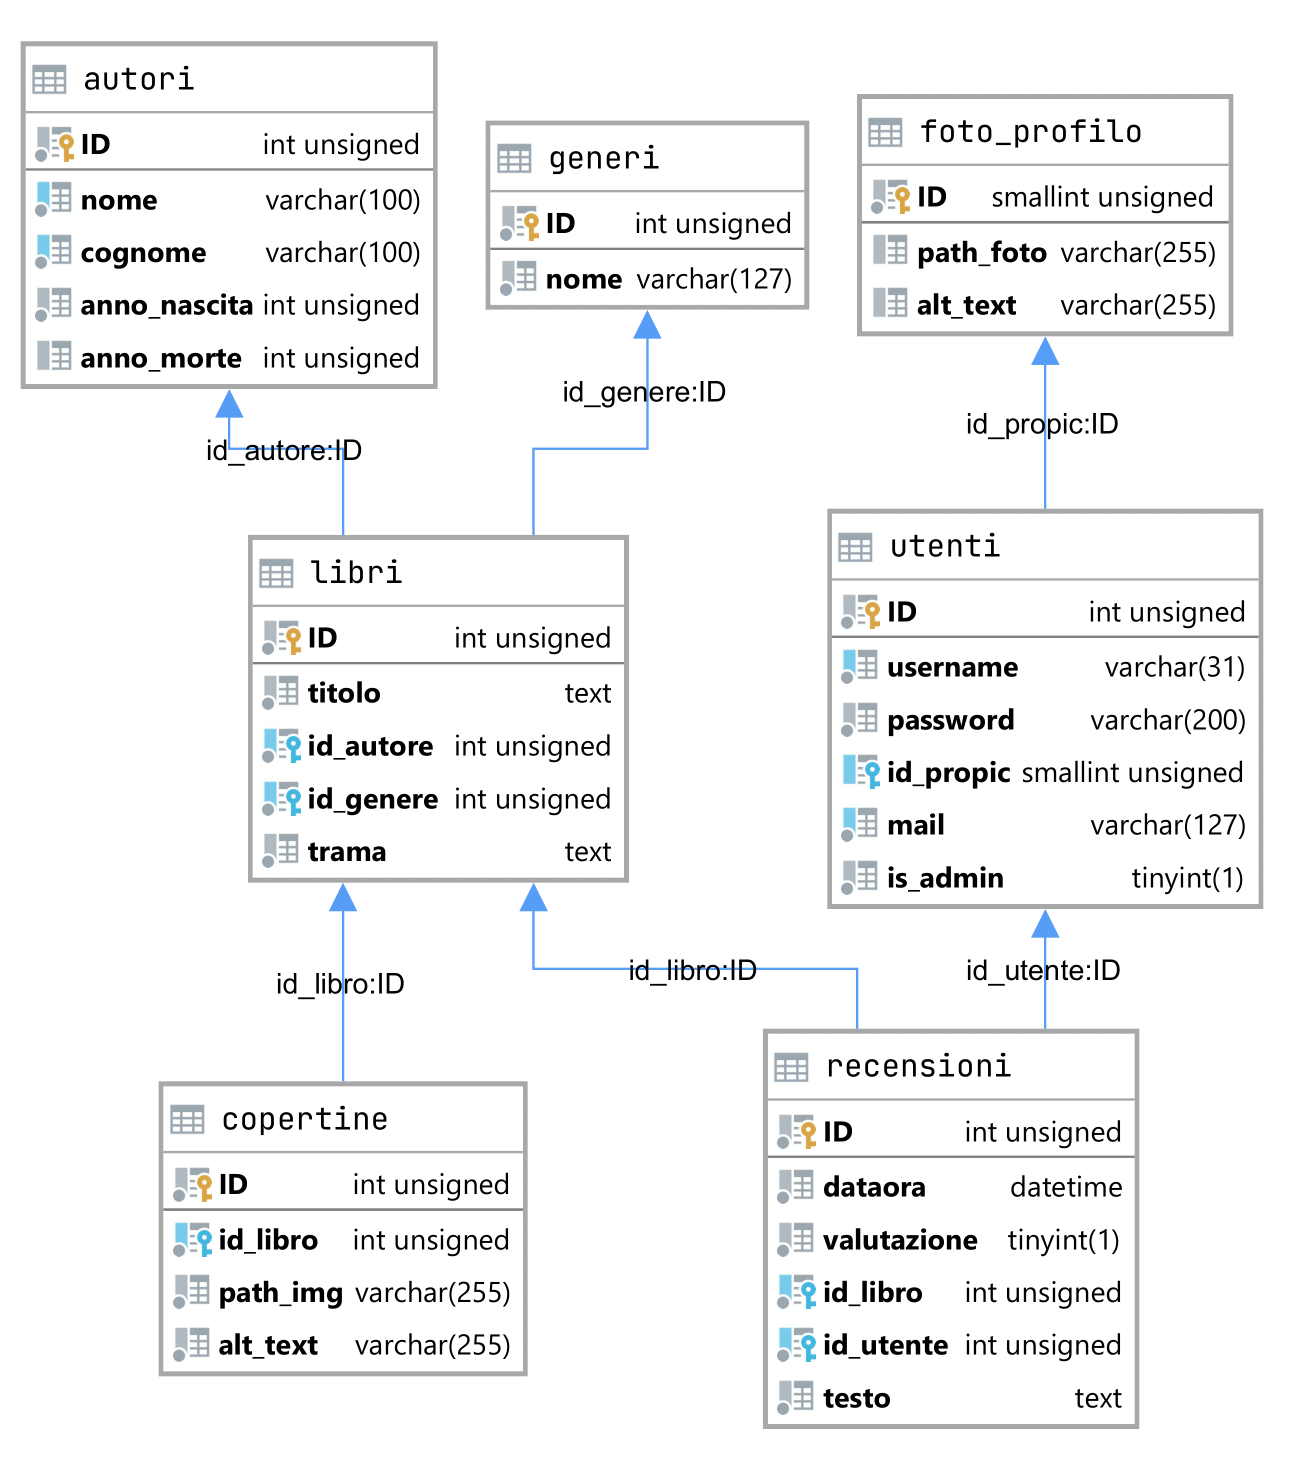
\includegraphics[width=0.6\textwidth]{../img/db_diagram/betweenthelines.png}
			\caption{Diagramma rappresentante la struttura del database}
		\end{figure}
	
	\subsubsection{PHP}
	\paragraph{Costruzione delle pagine} %TODO: simo
	
	\paragraph{Ricerca} %TODO:tonio
	
	\paragraph{Autenticazione}
	L'autenticazione è gestita con il sistema nativo di PHP delle sessioni. Quando un utente effettua con successo il login o la registrazione nel sistema, alcune delle sue informazioni vengono salvate all'interno della variabile superglobale \texttt{\_SESSION} per permetterne l'accesso da qualunque altro script. Quando un utente effettua il logout uno script si occupa di eliminare tutte le informazioni salvate in questa variabile. 
	
	\paragraph{Pagine di errore} %non sono sicuro che sta parte vada qua
	Per segnalare agli utenti errori nelle richieste al server sono state create delle pagine relative agli errori HTTP principali. Le pagine, il cui nome corrisponde al codice dell'errore che notificano sono:
	\begin{itemize}
		\item 400 - BAD REQUEST: quando l'URL della richiesta non rispetta alcuni criteri. Ritornato ad esempio in caso di una richiesta GET mal formata;
		\item 401 - UNAUTHORIZED: se per l'accesso alla pagina è necessaria l'autenticazione. Ritornato ad esempio provando ad entrare nel pannello utente se non è stata effettuata l'autenticazione;
		\item 403 - FORBIDDEN: nel caso in cui l'utente, pur se autenticato, non abbia i permessi necessari per eseguire l'operazione richiesta. Ad esempio nel caso in cui un utente non admin provasse ad aggiungere un libro;
		\item 404 - NOT FOUND: se la richiesta fatta al server non viene risolta.
	\end{itemize}
	
	\paragraph{Query al database}
	Per incentivare il riuso di codice si è scelto di implementare due funzioni con lo scopo di interagire con il database per la consultazione, l'inserimento e la modifica di dati:
	\begin{itemize}
		\item \texttt{queryDB(\$query)}: effettua una query e ritorna il risultato sotto forma di array o \texttt{NULL} se non va a buon fine;
		\item \texttt{insertDB(\$query)}: per effettuare query di inserimento e modifica al database: ritorna \texttt{true} se la query modifica almeno una tupla, \texttt{false} se nessuna riga viene modificata e \texttt{NULL} se la query non va a buon fine.
	\end{itemize}
	\paragraph{Validazione lato server}
	Le funzioni per la validazione dell'input lato server necessarie per la verifica dell'input inserito dall'utente agiscono in più modi:
	\begin{itemize}
		\item controllano, utilizzando il match con un espressione regolare, che l'input rispetti determinati criteri di accettazione. Le funzioni di questo tipo sono tutte contenute all'interno del file \texttt{regex\_checker}.Solitamente richiedono il match dell'intera stringa passata al metodo come parametro con l'espressione regolare definita;
		\item accertano che la stringa che gli viene passata stia all'interno di una determinato range stabilendo una dimensione minima, una massima o entrambe;
		\item confrontano due stringhe, accertando la loro uguaglianza;
		\item confrontano due numeri stabilendo quale è il minore, il maggiore o se sono uguali;
		\item confrontano un anno con l'anno attuale per controllare che il primo non sia futuro.
	\end{itemize}
	Il feedback della validazione è mostrato tramite messaggi di successo o di errore che compaiono in testa al form e forniscono una descrizione dettagliata di come risolvere il problema riscontrato.
	
	
	\subsubsection{Javascript}
	L'uso di javascript in questo progetto è mirato a fornire delle funzionalità non indispensabili alla fruizione dei contenuti presenti. Questa scelta è stata compiuta per non precludere l'uso del sito agli utenti ai quali, per incompatibilità del browser o per scelte personali, il codice javascript non funzionasse correttamente. In ogni caso qualora javascript risultasse disattivato viene mostrato al caricamento di ogni pagina che ne fa uso un messaggio di notifica mediante il tag \texttt{noscript}. 
	\paragraph{Validazione lato client}
	Per la validazione dell'input utente lato client sono stati implementati dei metodi che effettuano dei controlli sui parametri che gli vengono passati, accertando che questi rispettino determinati criteri. Questi metodi sono spesso equivalenti alle loro controparti lato server implementate con PHP. \\
	Degno di nota è \texttt{checkNome(name)} la cui funzione è quella di confrontare una stringa con una espressione regolare per assicurarsi che corrisponda ai criteri di un nome. Viene utilizzato ad esempio per la validazione di un genere e del nome e cognome di un autore. Questo controllo è più permissivo del suo corrispondente lato server (rifiuta solo i numeri) in quanto non è stato trovato un espediente per filtrare esclusivamente le lettere di ogni alfabeto codificate in UTF8, cosa possibile invece con le espressioni regolari messe a disposizione da PHP.\\
	I test di validazione vengono eseguiti quando il focus viene spostato da un campo di input e quando il form viene inviando, impedendone l'invio se almeno un test non viene superato.\\
	Il risultato della validazione è mostrato con messaggi di successo o di errore che precedono il campo di input al quale si riferiscono e forniscono una spiegazione esaustiva di come risolvere il problema riscontrato.
	
	\paragraph{Visualizzazione della preview dell'immagine di copertina} %todo:Luca
	
	\section{Testing}
	Il testing ha impegnato il gruppo non solo alla conclusione del progetto ma anche durante il suo sviluppo, in maniera da emendare prima possibile eventuali criticità.
	Sono stati utilizzati i seguenti strumenti:
	\begin{itemize}
		\item \href{https://validator.w3.org/}{Markup Validation Service} per verificare la conformità a \textit{XHTML 1.0 Strict} di ogni pagina del sito;
		\item \href{https://jigsaw.w3.org/css-validator/}{W3C CSS Validation Service} per i fogli di stile.
Si noti che le pagine sono fruibili anche senza fogli di stile in quanto sono state ridimensionate le immagini;
		\item il tool \textbf{Accessibility Insights for Web}, che offre un'analisi accurata di vari aspetti legati all'accessibilità e usabilità del sito; sono stati eseguiti test automatici (molto utili per verificare il rispetto del contrasto fra colori: 3:1 per testo grande e 4.5:1 per testo piccolo) ma anche test manuali tramite procedure guidate;
		\begin{figure}[h!]
			\caption{Accessibility Insights for Web - assessment in corso}
			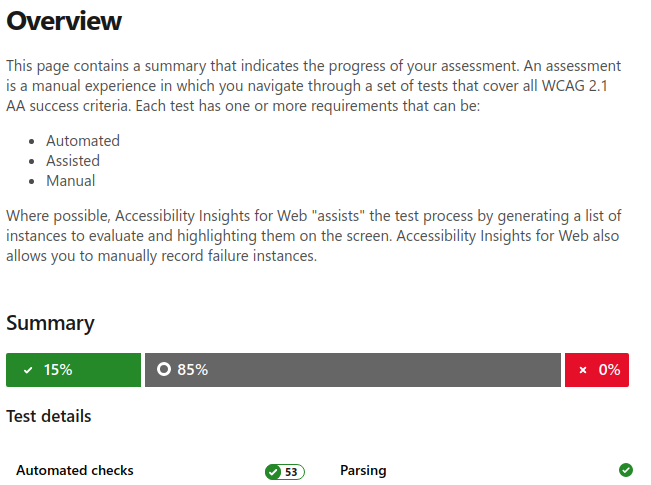
\includegraphics[width=0.7\textwidth]{../img/testing/AIFW.png}
		\end{figure}
		\item il tool \textbf{Total Validator} che ha segnalato la seguente criticità, poi emendata: alt troppo lunghi che sono stati accorciati (codice \textit{P888 - WCAG21 1.1.1 (A)});
		\item \textbf{Silktide - website accessibility simulator} che permette di comprendere quale sia la percezione del sito da parte di utenti fisicamente svantaggiati;
		\begin{figure}[h!]
			\caption{Silktide - test screen reader}
			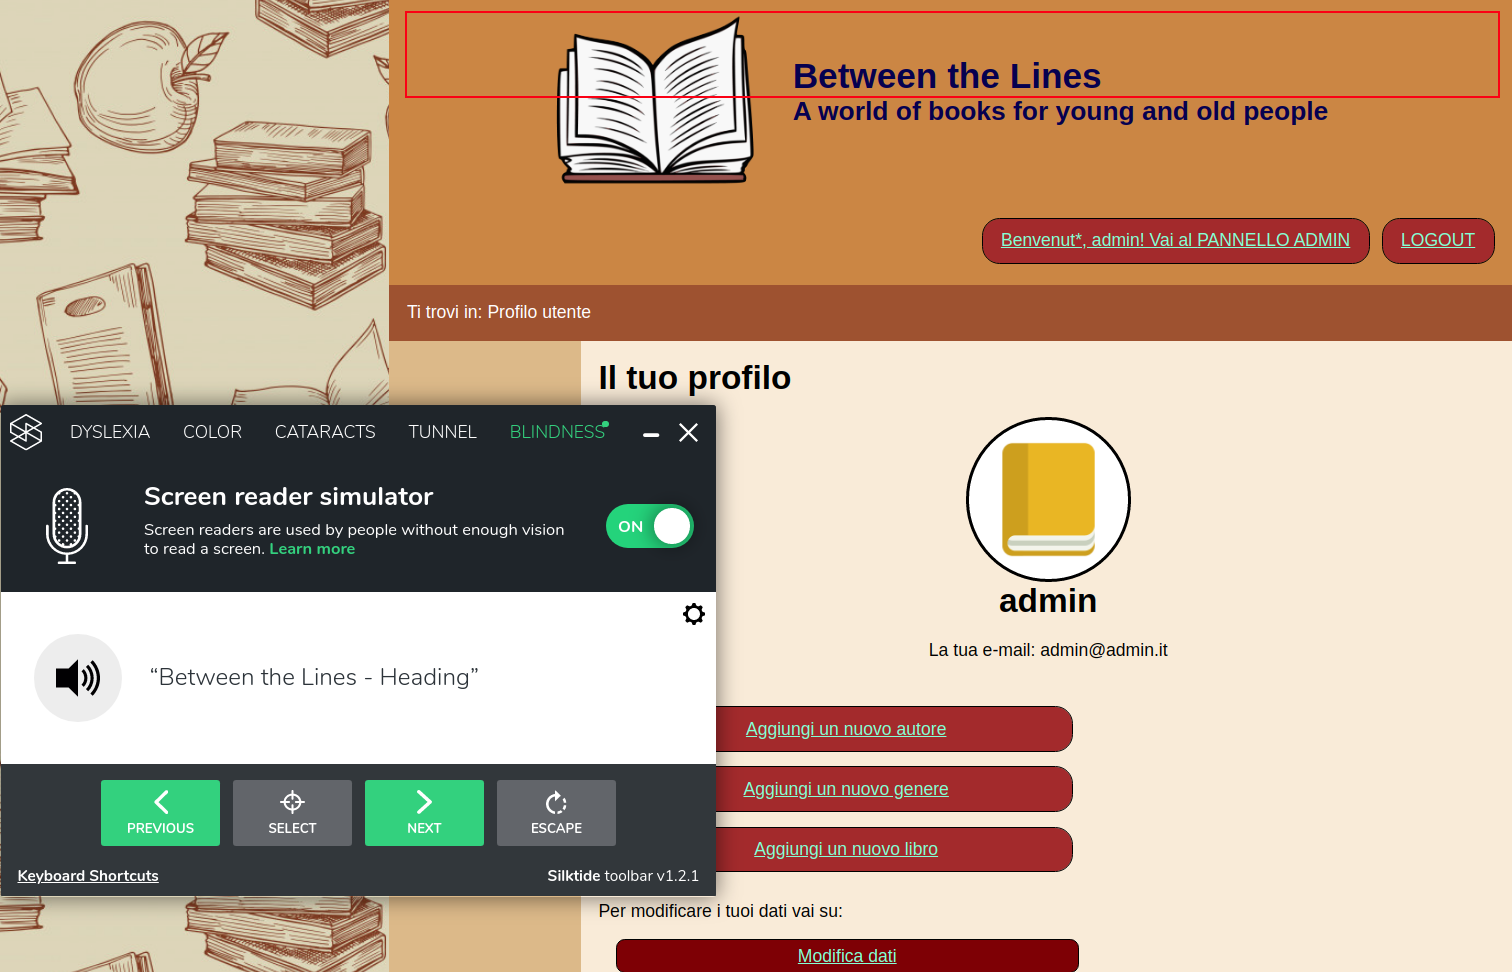
\includegraphics[width=0.7\textwidth]{../img/testing/silktide.png}
		\end{figure}
		\item \textbf{Web developer tool} per verificare l'input tramite form e la corretta visualizzazione delle immagini.
	\end{itemize}
	
	\section{Suddivisione del lavoro} %todo:Tutti - verificare e integrare
	Nella fase iniziale il gruppo ha lavorato assieme per la definizione dell'argomento del progetto, dei requisiti e della struttura del sito. Una volta definite le linee guida, i compiti sono stati suddivisi equamente fra i componenti del gruppo e in modo da garantire a tutti di affrontare ogni aspetto della realizzazione del sito (database, HTML, PHP, Javascript, CSS, testing). Periodicamente venivano indette delle riunioni per aggiornare il gruppo sul procedere dei lavori e risolvere eventuali problematiche.
	
	\begin{itemize}
		\item Antonio Badan: 
		\begin{itemize}
			\item popolamento database;
			\item realizzazione pagine (parti: HTML, PHP, Javascript, CSS, testing): chisiamo, contatti, ricerca, home;
			\item testing e validazione finale;
		\end{itemize}
		
		\item Simone De Renzis: 
		\begin{itemize}
			\item mockup sito;
			\item ossatura pagine HTML;
			\item realizzazione pagine (parti: HTML, PHP, Javascript, CSS, testing): dettagliLibro, sessione, pagine d'errore;
		\end{itemize}
		
		\item Francesco Trolese:
		\begin{itemize}
			\item realizzazione database;
			\item realizzazione pagine(parti: HTML, PHP, Javascript, CSS, testing): autenticazione utente / admin, inserimento autore - genere;
			\item definizione funzioni javascript;
		\end{itemize}
		
		\item Luca Veronese: 
		\begin{itemize}
			\item realizzazione database;
			\item ossatura pagine HTML;
			\item realizzazione pagine(parti: HTML, PHP, Javascript, CSS, testing): inserimento libro, pagine d'errore;
		\end{itemize}
	\end{itemize}
	
	\end{document}
